\chapter{Replication Results}
\label{chap:replication_results}
\section{Chapter Overview}

This chapter reports the results of the five dataset-specific replications. Its purpose is to document how closely the source-study workflows and results could be reconstructed before the thesis-specific validation and \gls{xai} extensions are considered.

Paper-style results reproduce the model families and analytical choices described in the source studies as closely as the available information permits. Where the source workflow raised a methodological concern, this chapter records the replicated procedure without treating its test result as an independently validated estimate. Thesis-specific corrected configurations are evaluated in Chapter~\ref{chap:validation_results}.

The heart disease, stroke, diabetes, and \gls{ckd} experiments use held-out test partitions. In contrast, the \gls{hbaone} experiment reproduces the full-cohort inferential logistic-regression analysis of the source study \citep{strack_impact_2014}. It therefore produces in-sample descriptive predictions rather than an estimate of out-of-sample predictive performance.

\section{Heart Disease Replication}

\subsection{Dataset and Experimental Result}

The Cleveland heart-disease dataset uses a binary outcome distinguishing the absence and presence of heart disease \citep{detrano_international_1989, khanna_comparative_2015}. After replacing the original missing-value marker and removing incomplete records, 297 observations remained. A fixed, stratified, near-equal partition produced 148 training observations and 149 test observations, with 13 predictors.

The replicated experiment compared logistic regression, three \gls{svm} kernels, and three neural-network variants, following the model scope of the source study \citep{khanna_comparative_2015}. As shown in Table~\ref{tab:heart_replication_results}, the backpropagation network achieved the highest held-out \gls{rocauc} at 0.924, while the \gls{grnn} achieved the highest held-out accuracy at 86.58\%. The radial-basis-function neural network performed substantially worse than the remaining models.

\begin{table}[htbp]
    \centering
    \small
    \caption{Held-out predictive performance of the models reconstructed in the Heart replication. Accuracy, F1 score, and \gls{rocauc} were calculated on the fixed test partition of 149 observations.}
    \label{tab:heart_replication_results}
    \begin{tabular}{@{}lrrr@{}}
        \toprule
        \textbf{Model} & \textbf{Accuracy} & \textbf{F1} & \textbf{\gls{rocauc}} \\
        \midrule
        Logistic regression (10-fold \gls{cv}) & 0.852 & 0.841 & 0.915 \\
        Linear \gls{svm} & 0.839 & 0.830 & 0.911 \\
        \gls{rbf} \gls{svm} & 0.859 & 0.840 & 0.912 \\
        Polynomial \gls{svm} & 0.785 & 0.760 & 0.880 \\
        Backpropagation neural network & 0.859 & 0.844 & 0.924 \\
        \gls{rbf} neural network & 0.758 & 0.670 & 0.648 \\
        \gls{grnn} & 0.866 & 0.850 & 0.913 \\
        \bottomrule
    \end{tabular}
\end{table}

The source study reported that logistic regression and the linear \gls{svm} performed strongly among the conventional classifiers. \gls{grnn} was the strongest neural-network configuration, while the \gls{rbf} network performed comparatively poorly \citep{khanna_comparative_2015}. The replication retained this broad pattern. Logistic regression and the \gls{svm} variants remained competitive, \gls{grnn} achieved the highest observed accuracy, and the \gls{rbf} network produced the weakest neural-network result. The reproduced rankings were not identical because the backpropagation network achieved the highest \gls{rocauc} in the present implementation.

The variation among the neural-network results demonstrates the difficulty of reproducing models from architecture labels alone. Reproducibility also depends on details such as parameter initialisation, optimisation, stopping criteria, and software implementation, which must be reported sufficiently for an analysis to be reconstructed \citep{collins_tripodai_2024}. The results are therefore interpreted as a procedural replication of the reported analytical approach rather than as evidence that every published numerical value can be recovered exactly.

\section{Stroke Replication}

\subsection{Outcome Imbalance and Feature Selection}

The original stroke dataset contained 5,110 observations, including one observation whose gender was recorded as ``Other'' \citep{wu_machine_2024}. The implemented preprocessing excluded this singleton category, leaving 5,109 observations. This exclusion avoided representing a categorical level from a single observation and should not be interpreted as indicating that the category itself was invalid. A stratified 80:20 partition produced 4,087 training observations and 1,022 test observations. Feature selection was performed using the training data only. Seven encoded predictors were retained: age, hypertension, heart disease, average glucose level, the \gls{bmi}-missingness indicator, and the two encoded levels of marital status. The evaluated model families followed the scope of the replicated stroke study \citep{wu_machine_2024}.

The outcome was strongly imbalanced. Consequently, accuracy alone could reward models that mainly predicted the majority class. This was visible in the descriptive model comparison: the neural network achieved accuracies of 0.951 before and 0.948 after feature selection, but the corresponding \gls{rocauc} values were 0.814 and 0.826. The difference between accuracy and discrimination motivated emphasis on \gls{rocauc} in the descriptive cross-model comparison. Precision, recall, and confusion-matrix-derived measures for the pre-specified
balanced logistic-regression configuration are reported separately in Chapter~\ref{chap:validation_results}.

Among the classical models evaluated on the selected features, logistic regression produced the highest observed test \gls{rocauc}, as shown in Table~\ref{tab:stroke_auc_results}.

\begin{table}[htbp]
    \centering
    \small
    \caption{Held-out \gls{rocauc} of the models evaluated in the Stroke replication after feature selection was performed using training data only.}
    \label{tab:stroke_auc_results}
    \begin{tabular}{@{}lr@{}}
        \toprule
        \textbf{Model} & \textbf{\gls{rocauc}} \\
        \midrule
        Logistic regression & 0.834 \\
        XGBoost & 0.786 \\
        \Gls{rf} & 0.720 \\
        \Gls{knn} & 0.693 \\
        \gls{svm} & 0.599 \\
        \Gls{dt} & 0.520 \\
        \bottomrule
    \end{tabular}
\end{table}

The source study emphasised the difficulty created by severe class imbalance and reported that the \gls{dnn} achieved substantially better discrimination than the conventional classifiers before feature selection \citep{wu_machine_2024}. The replication confirmed the importance of evaluating \gls{rocauc} rather than accuracy alone, but it did not reproduce the same model ranking. Logistic regression achieved the highest observed \gls{rocauc} among the replicated classical models, and the \gls{dnn} \gls{rocauc} increased slightly after training-only feature
selection rather than decreasing. These differences indicate that the reported ranking was sensitive to preprocessing, feature-selection, model-fitting, and implementation details.

The corrected branch differs from a full-data correlation-selection workflow because imputation, encoding, feature selection, and scaling were learned exclusively from the training partition. This reduces information leakage but also means that exact equality with results obtained through full-dataset preprocessing is neither expected nor methodologically required.

\section{Diabetes Replication}

\subsection{Preprocessing and Model Comparison}

The Pima Indians diabetes dataset contained 768 observations, comprising 500 negative and 268 positive outcomes \citep{chang_pima_2023}. Zero values in glucose, blood pressure, skin thickness, insulin, and \gls{bmi} were treated as missing because zero is not physiologically plausible for these measurements \citep{chang_pima_2023}. Following the stratified partition, median imputation was fitted using the training data and then applied to both partitions. The final partition contained 538 training observations and 230 test observations.

The replication compared \gls{dt}, \gls{rf}, and naive Bayes classifiers using the complete eight-feature dataset and the three- and five-feature subsets defined by the source study \citep{chang_pima_2023}. The best-performing configuration from each feature-set analysis is compared in Table~\ref{tab:diabetes_best_results}, allowing the effects of classifier choice and predictor-set size to be considered together.

\begin{table}[htbp]
    \centering
    \small
    \caption{Highest-accuracy model identified within each Diabetes feature configuration. Metrics were calculated on the common held-out test partition of 230 observations.}
    \label{tab:diabetes_best_results}
    \begin{tabular}{@{}llrrrr@{}}
        \toprule
        \textbf{Features} & \textbf{Model} & \textbf{Accuracy} & \textbf{Recall} & \textbf{F1} & \textbf{\gls{rocauc}} \\
        \midrule
        Three features & Naive Bayes & 0.739 & 0.525 & 0.583 & 0.818 \\
        Five features & \Gls{rf} & 0.752 & 0.600 & 0.627 & 0.816 \\
        Eight features & \Gls{rf} & 0.739 & 0.538 & 0.589 & 0.824 \\
        \bottomrule
    \end{tabular}
\end{table}

The full feature set produced the highest \gls{rocauc} among the three configurations, while the five-feature \gls{rf} achieved the highest accuracy, recall, and F1 score. The preferred configuration therefore depends on the evaluation objective. No single configuration performed best across every metric.

The source study reported that \gls{rf} achieved the highest accuracy using the complete eight-feature dataset, while naive Bayes achieved the highest accuracy in both reduced feature configurations \citep{chang_pima_2023}. The replication retained the full-dataset \gls{rf} pattern and identified naive Bayes as the highest-accuracy model for the three-feature configuration. In the five-feature analysis, however, \gls{rf} achieved a higher replicated accuracy than naive Bayes. The lower reproduced scores and the change in the five-feature ranking may reflect differences in software implementation, random data partitioning, and the use of training-fitted missing-value imputation \citep{collins_tripodai_2024, moons_probastai_2025}.

\section{Chronic Kidney Disease Replication}

The \gls{ckd} dataset contained 400 observations and 24 predictors after removal of the identifier and normalisation of the binary outcome. In the source-style workflow, missing-value imputation and categorical encoding were performed using the complete dataset before creating a stratified 70:30 partition. This preprocessing order was retained solely to reproduce the published workflow \citep{santhiya_chronic_2024}. The resulting metrics are presented in Table~\ref{tab:ckd_replication_results} and represent the paper-style analysis rather than the subsequently corrected evaluation.

\begin{table}[htbp]
    \centering
    \small
    \caption{Held-out performance obtained from the paper-style \gls{ckd} replication, in which imputation and categorical encoding were fitted before the train--test split. These results reproduce the source-style procedure and are not leakage-controlled estimates.}
    \label{tab:ckd_replication_results}
    \begin{tabular}{@{}lrrrr@{}}
        \toprule
        \textbf{Model} & \textbf{Accuracy} & \textbf{Precision} & \textbf{Recall} & \textbf{F1} \\
        \midrule
        \Gls{rf} & 0.992 & 0.987 & 1.000 & 0.993 \\
        Gradient boosting & 0.992 & 1.000 & 0.987 & 0.993 \\
        \Gls{dt} & 0.983 & 1.000 & 0.973 & 0.987 \\
        Gaussian naive Bayes & 0.942 & 1.000 & 0.907 & 0.951 \\
        \Gls{knn} & 0.650 & 0.739 & 0.680 & 0.708 \\
        \bottomrule
    \end{tabular}
\end{table}

The source study identified \gls{rf} as its preferred \gls{ckd} classifier \citep{santhiya_chronic_2024}. As shown in Table~\ref{tab:ckd_replication_results}, the replication broadly retained the strong performance of the tree-based ensemble methods. \Gls{rf} and gradient boosting achieved the same highest observed accuracy, while the \gls{dt} ranked immediately below them. \Gls{rf} was therefore not the unique empirical winner in the reproduced test results. Its performance nevertheless remained consistent with the source-study rationale used to pre-specify it for the subsequent analysis.

Because imputation and encoding were performed before the data partition, information from the eventual test observations contributed to the preprocessing transformations. The paper-style results therefore reproduce the implemented source workflow but should not be interpreted as leakage-controlled estimates of performance on unseen data \citep{collins_tripodai_2024, moons_probastai_2025}. The effect of correcting the preprocessing order is evaluated separately in Chapter~\ref{chap:validation_results}.

\section{\gls{hbaone} and Hospital Readmission Replication}

\subsection{Cohort Reconstruction}

The \gls{hbaone} study was reconstructed as an observational full-cohort analysis rather than as a held-out classification benchmark \citep{strack_impact_2014}. The cohort was constructed by retaining the first eligible encounter for each patient, excluding records in which gender was recorded as ``Unknown/Invalid'', excluding death- or hospice-associated discharge dispositions, and deriving the grouped covariates described in the source study. The resulting analytical cohort contained 69,970 observations.

Within this cohort, 6,277 encounters (8.97\%) were followed by readmission within 30 days. No \gls{hbaone} test was recorded for 57,125 observations (81.64\%). The unadjusted 30-day readmission proportion was 9.10\% when no test was performed, 8.61\% for a normal result, 8.58\% for a high result followed by a medication change, and 7.38\% for a high result without a medication change. These percentages describe unadjusted associations within the reconstructed cohort. They do not estimate causal effects of \gls{hbaone} testing or medication changes.

Figure~\ref{fig:hba1c_replication_figure1} reconstructs the principal interaction figure reported by \citet{strack_impact_2014}. Predicted readmission probabilities were calculated from the replicated final logistic-regression model using the mean time in hospital and the reference levels of the remaining covariates.

The reconstruction retained the principal qualitative finding reported by the source study. The association between \gls{hbaone} category and predicted readmission probability differed according to the primary-diagnosis group \citep{strack_impact_2014}. The diabetes and respiratory groups showed lower predicted probabilities for some measured-\gls{hbaone} categories than for the category in which no test was recorded. The circulatory group followed a different pattern. Confidence intervals overlapped substantially across several comparisons. The reconstruction therefore supports procedural agreement with the published interaction pattern, but it is not presented as an exact numerical reproduction of every predicted probability.

\begin{figure}[H]
    \centering
    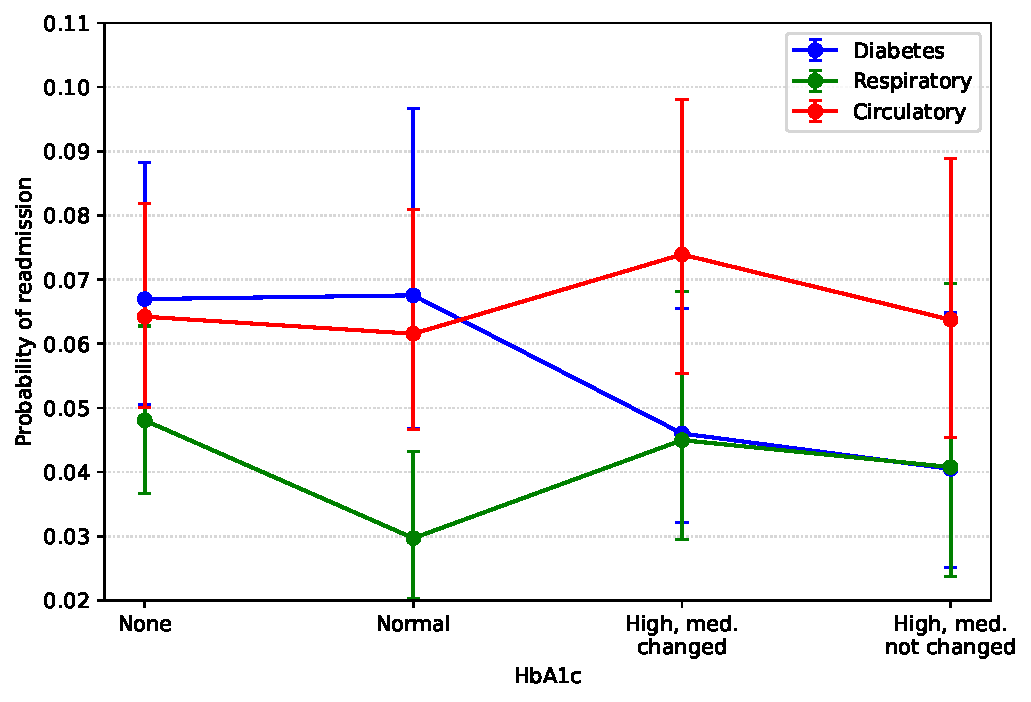
\includegraphics[width=0.82\textwidth]
    {images/results/hba1c_replication_figure1.pdf}
    \caption{Reconstruction of the adjusted readmission-probability comparison reported by \citet{strack_impact_2014}. Points show predicted probabilities for the four \gls{hbaone} categories across three primary-diagnosis groups. Error bars show 95\% inferential confidence intervals. Predictions are conditional on the reference covariate profile and mean time in hospital. They are not estimates of held-out predictive performance or causal effects.}
    \label{fig:hba1c_replication_figure1}
\end{figure}

\FloatBarrier

\section{Replication Findings in Relation to RQ1}

The five published workflows could be reconstructed at the level of datasets, broad preprocessing stages, model families, and analytical objectives. Exact numerical reproduction was not always possible. Differences arose from incomplete reporting of random procedures, implementation-specific neural-network architectures, ambiguous preprocessing order, feature-selection leakage, and the distinction between predictive and inferential study designs.

Three general findings emerged. First, the final predictive configurations separated the data before fitting learned preprocessing operations, even when a paper-style branch was retained for comparison. This prevented information from the test partition from influencing preprocessing and model development. Second, held-out test performance was not used retrospectively to select the models for \gls{xai} analysis. Those models were pre-specified using the source-study rationale and the corrected analytical design. Third, differences among the tasks affected how their results could be interpreted. The four held-out binary classifiers and the full-cohort \gls{hbaone} regression do not represent equivalent predictive experiments.

These findings answer RQ1 by demonstrating that procedural replication was achievable across the five studies. Exact numerical reproducibility was nevertheless constrained by reporting detail, methodological ambiguity, and implementation-specific decisions. The reconstructed workflows provide a documented foundation for the evaluation of the final analytical configurations presented in Chapter~\ref{chap:validation_results}.